\documentclass{article}
\usepackage[italian]{babel}
\usepackage[T1]{fontenc}
\usepackage{graphicx}
\usepackage[utf8x]{inputenc}
\usepackage{amsmath}
\usepackage{amsthm}
\usepackage{hyperref}
\date{Novembre 2015}
\author{Francesco Sacco, Lorenzo Cavuoti}
\title{Usi non lineari dell'OpAmp}

\begin{document}
	\maketitle
	\section{Amplificatore di carica}
	\subsection{Teoria}
		Per spiegare il circuito dell'amplificatore di carica è meglio analizzarlo con i suoi due sotto-circuiti separatamente, e poi vedere come si incastrano assieme.\newline

		Il primo sottocircuito è quello che è collegato al voltaggio in ingresso $V_S$, esso si può vedere nella figura \ref{fig:circ1}
		\begin{figure}
			\label{fig:circ1}
			\centering
			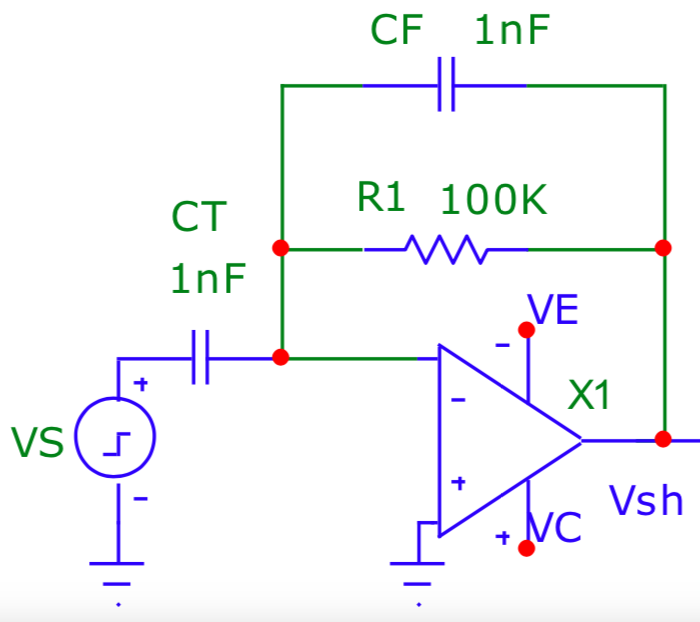
\includegraphics[width=70mm]{immagini/circ1.png}
			\caption{sotto-circuito 1}
		\end{figure}
		, risolvere il circuito equivale a risolvere questo sistema di 3 equazioni
		\begin{equation}
			\begin{cases}
				V_s-V_-=\frac{Q_T}{C_T}\\
				V_--V_{sh}=I_1R_1\\
				V_--V_{sh}=\frac{Q_F}{C_F}
			\end{cases}
		\end{equation}

\end{document}